\chapter{Unity} \label{appendice_Unity}

\section{Utilizzare la libreria}

La distribuzione della libreria realizzata per Unity viene effettuata attraverso la generazione di un \textit{Asset packages} ossia collezione di file e dati, realizzati da progetti Unity, compressi e memorizzati in un unico file, simile ad una cartella compressa. 
All'interno del package, la struttura dei file e i metadati rimangono gli stessi dell'originale così da rendere possibile la distribuzione del codice sorgente e delle dipendenze esterne.

\medskip

La libreria prodotta, \textit{Synapsis.unitypackage}, è disponibile sul repository del middleware (sezione \ref{materiale_online}) e per importarla è necessario creare un nuovo progetto Unity, da menu "Assets"->"Import Package"->"Custom Package" e selezionare la libreria.


\section{Realizzare Script custom}

Come spiegato nella sezione \ref{libreria_unity}, la classe \textit{SynapsisBody} è uno script che contiene le funzionalità di collegamento al middleware. Per realizzare uno script custom è sufficiente creare una nuova classe che estenda \textit{SynapsisBody}.

\lstinputlisting[caption=Esempio di script che estende SynapsisBody,language={[Sharp]C}]{code/Test.cs}

I metodi \textit{CounterpartEntityReady} e \textit{CounterpartEntityUnready} vengono utilizzati per conoscere lo stato di collegamento con la controparte mente. Questi metodi vengono automaticamente invocati in base alle informazioni ricevute dal middleware.

\medskip

Collegando lo script sopra elencato al GameObject compaiono, nella sezione "Inspector" di Unity", le configurazioni necessarie per definire il collegamento al middleware, nell'editor di Unity.

\begin{figure}[H]
\centering
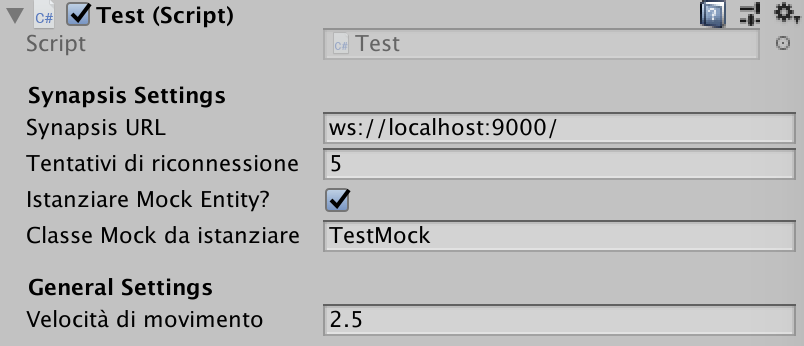
\includegraphics[width=\textwidth]{figures/Unity_Test_editor.png}
\caption{Configurazioni dello Script Test che estende SynapsisBody}
\end{figure}

Le configurazioni riguardano il collegamento al middleware, la necessità di instanziare una MockEntity e la velocità di movimento dell'entità (se deve effettuare spostamenti nell'ambiente).